\subsubsection{Secure Element} \label{section:counter-replace-encryption-key-local}

idea: store key at secure place where it is not exposed but delivers decrypted output for an input, best suitable for this task smartcard


can either be mounted in the sdcard slot or using an adapter for the usb interface
accessed over reads and writes to the filesystem
since it has to be small as a sd card and powered by the host system its hardware capabilities are restrained as well \cite{stSe} with power as low as 25MHz complexe calculations would take too much time

simple tasks (beschreiben)

unbestechlich, jedoch boolean abfrage immer crackbar, deswegen andere sachen machen zB verschlüsseln

encrypted strings from the application can be decrypted by the secure element
store property settings on it

encryption key can be stored on

no complexe tasks since low power

\begin{figure}[h]
    \centering
    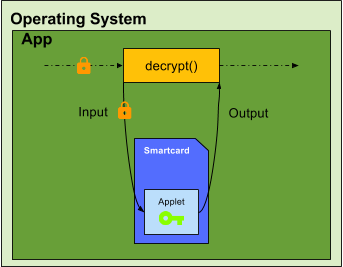
\includegraphics[width=0.8\textwidth]{data/encryptionKeySmart.png}
    \caption{Decryption by using a smartcard}
    \label{fig:encryptionKeySmart}
\end{figure}


same as internet service but extra hardare has to be bought
people are lazy and do not want to have extra hardware
when integrated into phone, it will take a long time until each phone supports it, e.g. was not able to use it on Nexus 6P and Nexus 7, Linux did not recognize it but mass storage was enabled, Nexus7 said OTG available but it did not work
many different implementation fragmentate the market, there is not one single solution to focus on and push for market wide accepted solution
solution which are out there have major security flaws, smartcard itself can be attacked

have problems on their own, nur so sicher wie das secure element
DAP Verification .... normalerweise muss jede Applet, die auf so ein Secure Element/Smartcard etc. kommt mit ner Signatur unterschrieben sein ...
%\url{http://www.win.tue.nl/pinpasjc/docs/Card%20Spec%20v2.1.1%20v0303.pdf}


Waehrend ich Exploits finden konnte, die Dir erw. Zugriff geben, wenn du Applets installieren kannst, u.a.
%\url{https://www.cs.ru.nl/E.Poll/papers/cardis08.pdf}
%\url{http://www.uclouvain.be/crypto/wissec2009/static/13.pdf}​
